%           ******************************************************
%          **   course         : Advanced Computer Architecture  **
%         ***   Presentation   : 03                              ***
%        ****   Topic          : Structure of Motherboard        ****
%        ****   AUTHOR         : Reza Adinepour                  ****
%         ***   Student ID:    : 402131055                       ***
%          **   Github         : github.com/rezaAdinepour/       **
%           ******************************************************

\documentclass[
	12pt, % Set the default font size, options include: 8pt, 9pt, 10pt, 11pt, 12pt, 14pt, 17pt, 20pt
	%t, % Uncomment to vertically align all slide content to the top of the slide, rather than the default centered
	%aspectratio=169, % Uncomment to set the aspect ratio to a 16:9 ratio which matches the aspect ratio of 1080p and 4K screens and projectors
]{beamer}

\graphicspath{{Images/}{./}} % Specifies where to look for included images (trailing slash required)

\usepackage{booktabs} % Allows the use of \toprule, \midrule and \bottomrule for better rules in tables
\usepackage{subcaption}

%----------------------------------------------------------------------------------------
%	SELECT LAYOUT THEME
%----------------------------------------------------------------------------------------

% Beamer comes with a number of default layout themes which change the colors and layouts of slides. Below is a list of all themes available, uncomment each in turn to see what they look like.

%\usetheme{default}
%\usetheme{AnnArbor}
%\usetheme{Antibes}
%\usetheme{Bergen}
%\usetheme{Berkeley}
%\usetheme{Berlin}
\usetheme{Boadilla}
%%%%%%%%%\usetheme{CambridgeUS}
%\usetheme{Copenhagen}
%\usetheme{Darmstadt}
%\usetheme{Dresden}
%\usetheme{Frankfurt}
%\usetheme{Goettingen}
%\usetheme{Hannover}
%\usetheme{Ilmenau}
%\usetheme{JuanLesPins}
%\usetheme{Luebeck}
%%%%%\usetheme{Madrid}
%\usetheme{Malmoe}
%\usetheme{Marburg}
%\usetheme{Montpellier}
%\usetheme{PaloAlto}
%\usetheme{Pittsburgh}
%\usetheme{Rochester}
%\usetheme{Singapore}
%\usetheme{Szeged}
%\usetheme{Warsaw}

%----------------------------------------------------------------------------------------
%	SELECT COLOR THEME
%----------------------------------------------------------------------------------------

% Beamer comes with a number of color themes that can be applied to any layout theme to change its colors. Uncomment each of these in turn to see how they change the colors of your selected layout theme.

%\usecolortheme{albatross}
\usecolortheme{beaver}
%\usecolortheme{beetle}
%\usecolortheme{crane}
%\usecolortheme{dolphin}
%\usecolortheme{dove}
%\usecolortheme{fly}
%%%%%%%%\usecolortheme{lily}
%\usecolortheme{monarca}
%\usecolortheme{seagull}
%\usecolortheme{seahorse}
%\usecolortheme{spruce}
%\usecolortheme{whale}
%\usecolortheme{wolverine}

%----------------------------------------------------------------------------------------
%	SELECT FONT THEME & FONTS
%----------------------------------------------------------------------------------------

% Beamer comes with several font themes to easily change the fonts used in various parts of the presentation. Review the comments beside each one to decide if you would like to use it. Note that additional options can be specified for several of these font themes, consult the beamer documentation for more information.

\usefonttheme{default} % Typeset using the default sans serif font
%\usefonttheme{serif} % Typeset using the default serif font (make sure a sans font isn't being set as the default font if you use this option!)
%\usefonttheme{structurebold} % Typeset important structure text (titles, headlines, footlines, sidebar, etc) in bold
%\usefonttheme{structureitalicserif} % Typeset important structure text (titles, headlines, footlines, sidebar, etc) in italic serif
%\usefonttheme{structuresmallcapsserif} % Typeset important structure text (titles, headlines, footlines, sidebar, etc) in small caps serif

%------------------------------------------------

%\usepackage{mathptmx} % Use the Times font for serif text
\usepackage{palatino} % Use the Palatino font for serif text

%\usepackage{helvet} % Use the Helvetica font for sans serif text
\usepackage[default]{opensans} % Use the Open Sans font for sans serif text
%\usepackage[default]{FiraSans} % Use the Fira Sans font for sans serif text
%\usepackage[default]{lato} % Use the Lato font for sans serif text

%----------------------------------------------------------------------------------------
%	SELECT INNER THEME
%----------------------------------------------------------------------------------------

% Inner themes change the styling of internal slide elements, for example: bullet points, blocks, bibliography entries, title pages, theorems, etc. Uncomment each theme in turn to see what changes it makes to your presentation.

%\useinnertheme{default}
\useinnertheme{circles}
%\useinnertheme{rectangles}
%\useinnertheme{rounded}
%\useinnertheme{inmargin}

%----------------------------------------------------------------------------------------
%	SELECT OUTER THEME
%----------------------------------------------------------------------------------------

% Outer themes change the overall layout of slides, such as: header and footer lines, sidebars and slide titles. Uncomment each theme in turn to see what changes it makes to your presentation.

\useoutertheme{default}
%\useoutertheme{infolines}
%\useoutertheme{miniframes}
%\useoutertheme{smoothbars}
%\useoutertheme{sidebar}
%\useoutertheme{split}
%\useoutertheme{shadow}
%\useoutertheme{tree}
%\useoutertheme{smoothtree}

%\setbeamertemplate{footline} % Uncomment this line to remove the footer line in all slides
%\setbeamertemplate{footline}[page number] % Uncomment this line to replace the footer line in all slides with a simple slide count

%\setbeamertemplate{navigation symbols}{} % Uncomment this line to remove the navigation symbols from the bottom of all slides

%----------------------------------------------------------------------------------------
%	PRESENTATION INFORMATION
%----------------------------------------------------------------------------------------

\title[Motherboard structure]{Motherboard Structure} % The short title in the optional parameter appears at the bottom of every slide, the full title in the main parameter is only on the title page

\subtitle{Everything you need to know about this structure} % Presentation subtitle, remove this command if a subtitle isn't required

\author[Reza Adinepour]{Reza Adinepour} % Presenter name(s), the optional parameter can contain a shortened version to appear on the bottom of every slide, while the main parameter will appear on the title slide

\institute[AUT]{Amirkabir University of Technology\\ (Tehran Polytechnic) \\ \smallskip \textit{\href{mailto:adinepour@aut.ac.ir}{adinepour@aut.ac.ir}}} % Your institution, the optional parameter can be used for the institution shorthand and will appear on the bottom of every slide after author names, while the required parameter is used on the title slide and can include your email address or additional information on separate lines

\date[\today]{Computer Engineering Department \\ \today} % Presentation date or conference/meeting name, the optional parameter can contain a shortened version to appear on the bottom of every slide, while the required parameter value is output to the title slide

%----------------------------------------------------------------------------------------

\begin{document}

%----------------------------------------------------------------------------------------
%	TITLE SLIDE
%----------------------------------------------------------------------------------------

\begin{frame}
	\titlepage % Output the title slide, automatically created using the text entered in the PRESENTATION INFORMATION block above
	\centering
\includegraphics[scale=0.13]{Images/Logo/logo2.png}
\end{frame}

%----------------------------------------------------------------------------------------
%	TABLE OF CONTENTS SLIDE
%----------------------------------------------------------------------------------------

% The table of contents outputs the sections and subsections that appear in your presentation, specified with the standard \section and \subsection commands. You may either display all sections and subsections on one slide with \tableofcontents, or display each section at a time on subsequent slides with \tableofcontents[pausesections]. The latter is useful if you want to step through each section and mention what you will discuss.

\begin{frame}
	\frametitle{Presentation Overview} % Slide title, remove this command for no title
	
	\tableofcontents % Output the table of contents (all sections on one slide)
	%\tableofcontents[pausesections] % Output the table of contents (break sections up across separate slides)
\end{frame}

%----------------------------------------------------------------------------------------
%	PRESENTATION BODY SLIDES
%----------------------------------------------------------------------------------------

\section{What is Motherboard?} % Sections are added in order to organize your presentation into discrete blocks, all sections and subsections are automatically output to the table of contents as an overview of the talk but NOT output in the presentation as separate slides

%------------------------------------------------

\subsection{Anatomy of a motherboard}

\begin{frame}
	\frametitle{What is motherboard?}
	
	Your computer is made of different electrical boards and circuits. All these circuits are offered to the customer \alert{in a package called motherboard}
	
	\bigskip % Vertical whitespace
	
	% Quote example
	\begin{quote}
		Essentially, it's like the central hub that enables all the parts of a computer to work together.\\
		--- \textcolor{blue}{ChatGPT}
	\end{quote}
	
	\bigskip % Vertical whitespace
	
	This part of the computer is as important as the most important components of the computer, i.e. CPU and GPU.
\end{frame}

%------------------------------------------------

\subsection{Standard Size}

\begin{frame}
	\frametitle{Standard Size}
	\framesubtitle{of motherboard} % Optional subtitle
	
	The main motherboard sizes are as follows:
	\begin{itemize}
		\item Standard ATX ($244mm \times 305mm$)
		\item Micro ATX ($244mm \times 244mm$)
		\item Mini ITX ($150mm \times 150mm$)
	\end{itemize}
	
	\bigskip % Vertical whitespace
	
	\begin{figure}
		\centering
		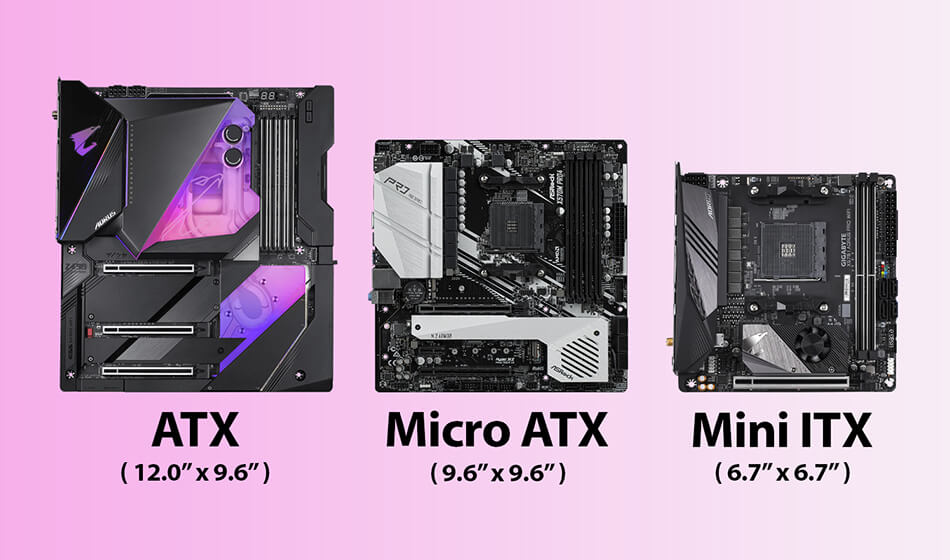
\includegraphics[width=0.5\linewidth]{Images/img1.jpg}
		\caption{Standard motherboard size}
		\label{motherboard size}
	\end{figure}
\end{frame}

%------------------------------------------------

\subsection{Main blocks}

\begin{frame}
	\frametitle{Main blocks}
	\framesubtitle{Figures}
	\begin{figure}
		\centering
		\begin{subfigure}[b]{0.3\textwidth}
			\centering
			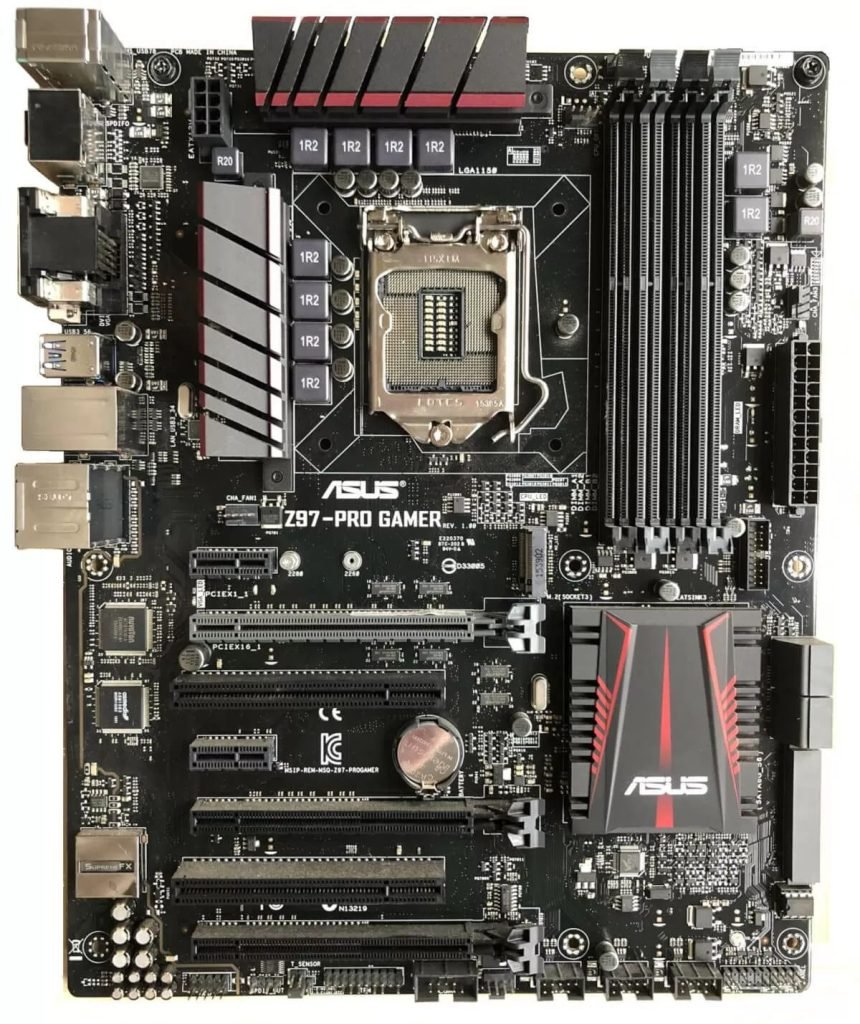
\includegraphics[width=1.1\linewidth]{Images/img2.jpg}
			\caption{Standard ATX motherboard Z97 pro gaming}
			\label{Z97}
		\end{subfigure}
		\hfill
		\begin{subfigure}[b]{0.3\textwidth}
			\centering
			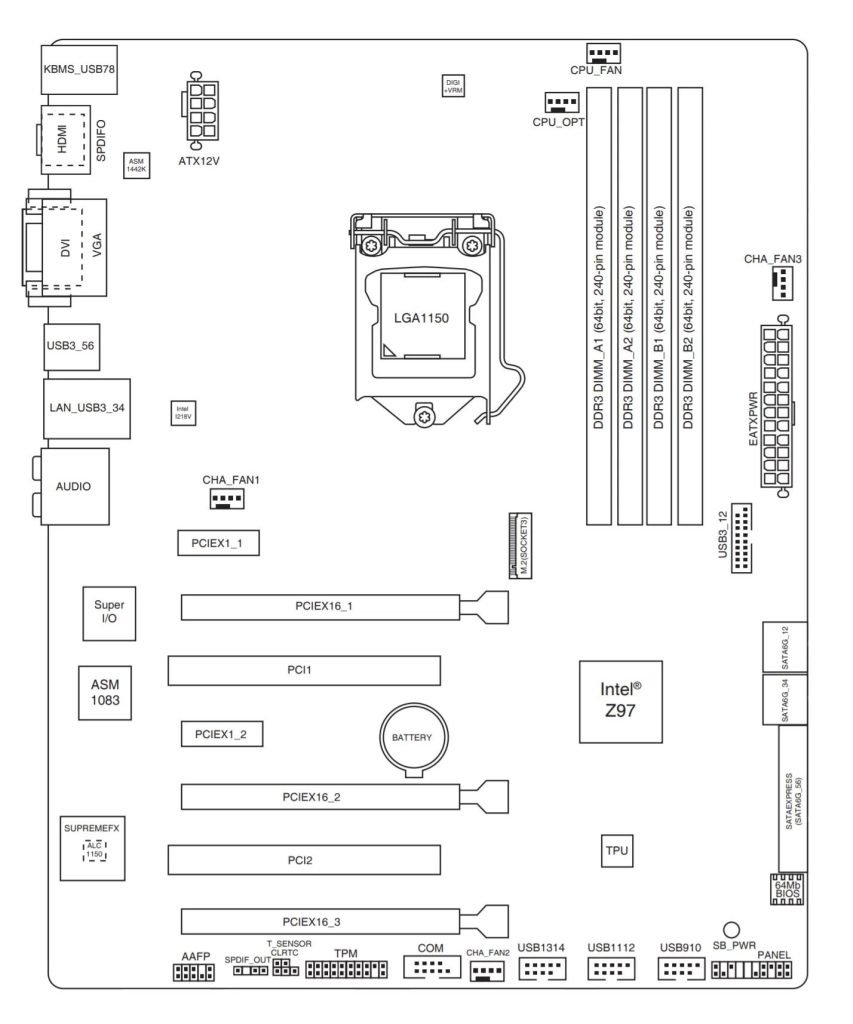
\includegraphics[width=1.1\linewidth]{Images/img3.jpg}
			\caption{Block diagram of Z97 pro gaming motherboard}
			\label{Z97 sch}
		\end{subfigure}
	\end{figure}
\end{frame}




\begin{frame}
	\frametitle{Main blocks}
	\framesubtitle{Overview}
	in (\textcolor{blue}{figure \ref{Z97 sch}}) we can see this blocks: 
	\begin{itemize}
		\item LGA 1150
		\item RAM slots
		\item M2 connector
		\item HDMI connector
		\item VGA connector
		\item Audio connector
		\item USB connector
		\item ...
	\end{itemize}
\end{frame}





\begin{frame}
	\frametitle{Main blocks}
	\framesubtitle{LGA 1150}
	
	\textcolor{blue}{L}and \textcolor{blue}{G}rid \textcolor{blue}{A}rray or LGA is the CPU socket that named by Intel.
	
	The number 1150 indicates number of socket pins.
	
	\begin{figure}
		\centering
		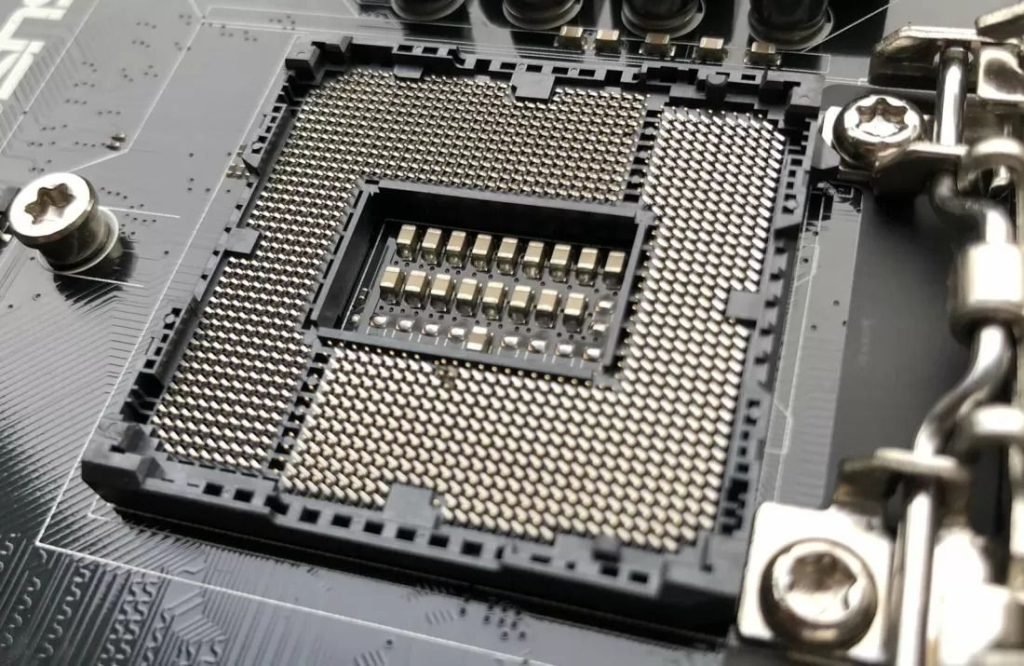
\includegraphics[width=0.65\linewidth]{Images/img4.jpg}
		\caption{LGA socket}
		\label{LGA socket}
	\end{figure}
\end{frame}






\begin{frame}
	\frametitle{Main blocks}
	\framesubtitle{Ram slots}
	
	The nearest slots and sockets to the CPU are DRAM slots, that called \textcolor{blue}{system memory}.
	
	These parts are directly connected to the CPU and the number of DRAMs in each motherboard depends on the type of CPU.
	
	\begin{figure}
		\centering
		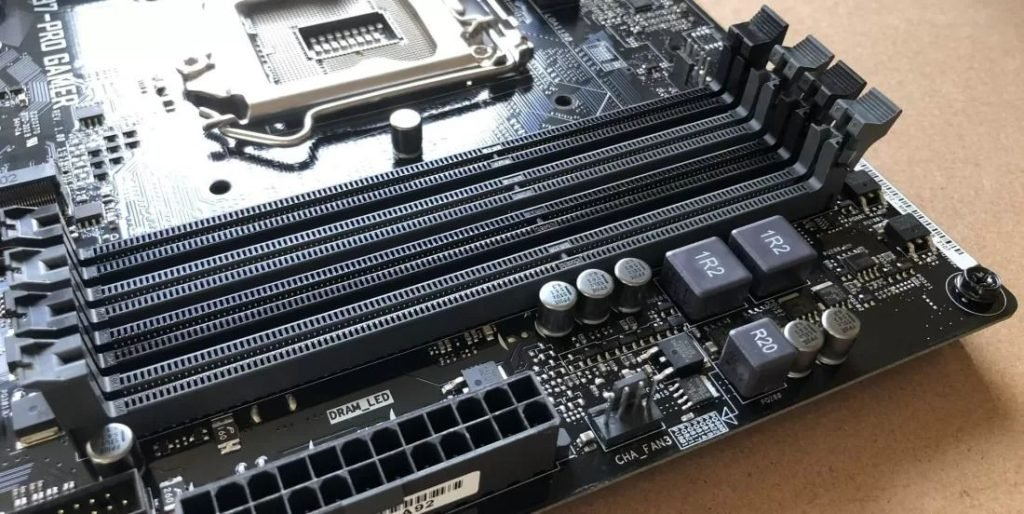
\includegraphics[width=0.7\linewidth]{Images/img5.jpg}
		\caption{RAM slots}
		\label{RAM slots}
	\end{figure}
\end{frame}





\begin{frame}
	\frametitle{Main blocks}
	\framesubtitle{M2 connector}
	
	This socket is used to connect the SSD memory to the motherboard.
	
	\begin{figure}
		\centering
		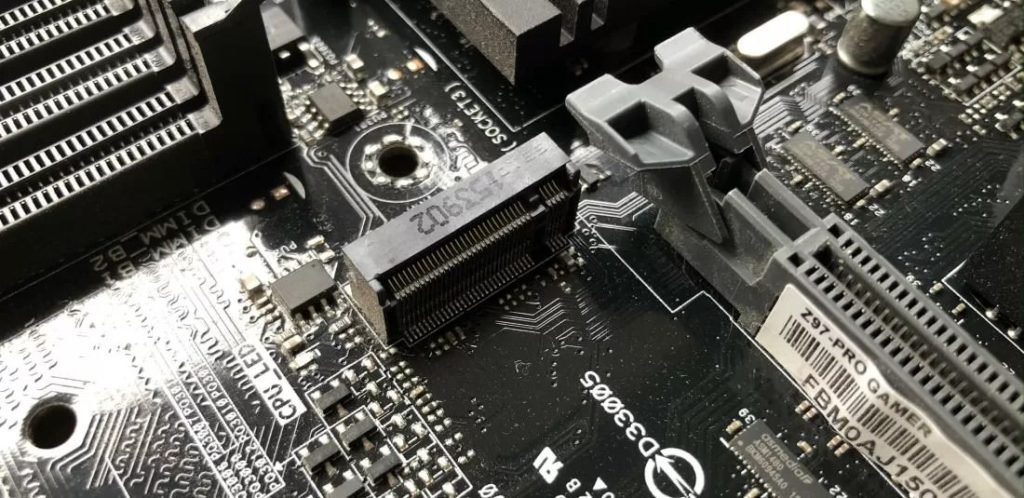
\includegraphics[width=0.8\linewidth]{Images/img7.jpg}
		\caption{M2 connector}
		\label{M2 connector}
	\end{figure}
\end{frame}




\begin{frame}
	\frametitle{Port \& connections}
	\framesubtitle{I/O connectors}
	
	This motherboard has these I/Os:
	\begin{itemize}
		\item PS/2: \textit{to connect keyboard and mouse}
		\item DVI-D: \textit{to connect to the GPU}
		\item VGA: \textit{to connect old displays device}
		\item HDMI
		\item Ethernet
		\item USB2 and USB3
		\item Audio jacks
	\end{itemize}
	
	\begin{figure}
		\centering
		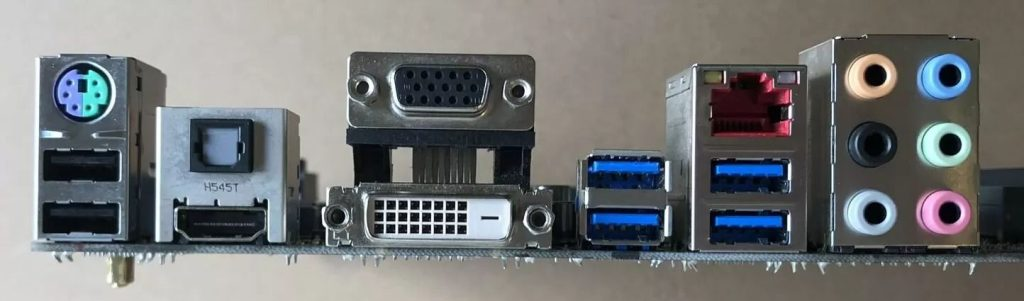
\includegraphics[width=0.6\linewidth]{Images/img6.jpg}
		\caption{I/O connector}
		\label{I/O connector}
	\end{figure}
\end{frame}

%------------------------------------------------

\subsection{North bridge and south bridge}

\begin{frame}
	\frametitle{North \& south bridge}
	\begin{enumerate}
		\item The NB and SB are components of older motherboard architectures.
		\item The NB manages communication between the processor, memory, and high-speed components like the graphics card. 
		\item The SB handles connections to slower peripherals like USB, SATA, and audio devices.
	\end{enumerate}
%	SATA stands for Serial Advanced Technology Attachment. It is a computer bus interface that is commonly used for connecting storage devices, such as hard disk drives (HDDs) and solid-state drives (SSDs), to the motherboard
	
	\alert{However, in modern motherboard designs, the functions of the North and South bridges have been integrated into a single chip called the Platform Controller Hub (PCH). (\textcolor{blue}{check figure \ref{Z97}})}
\end{frame}


\begin{frame}
	\frametitle{North \& south bridge}
	\framesubtitle{Figure}
	\begin{figure}
		\centering
		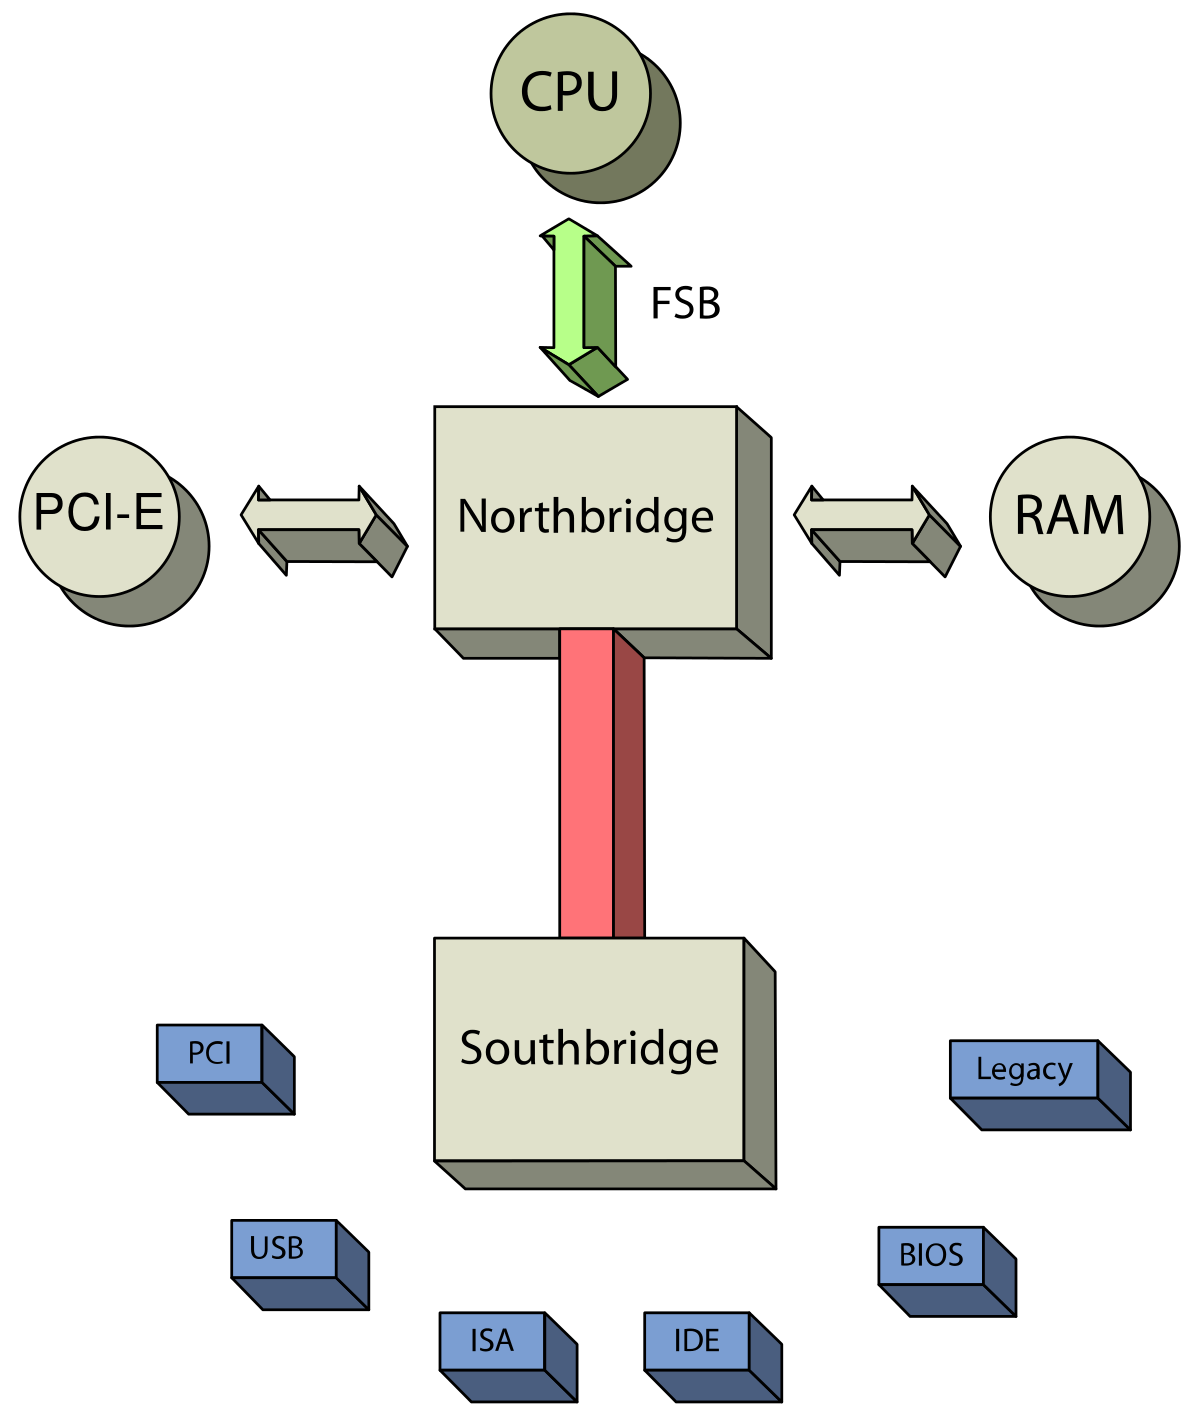
\includegraphics[width=0.45\linewidth]{Images/img8.png}
		\caption{NB and SB}
		\label{NB and SB}
	\end{figure}
\end{frame}




\begin{frame}
	\frametitle{North \& south bridge}
	\framesubtitle{Figure}
	\begin{figure}
		\centering
		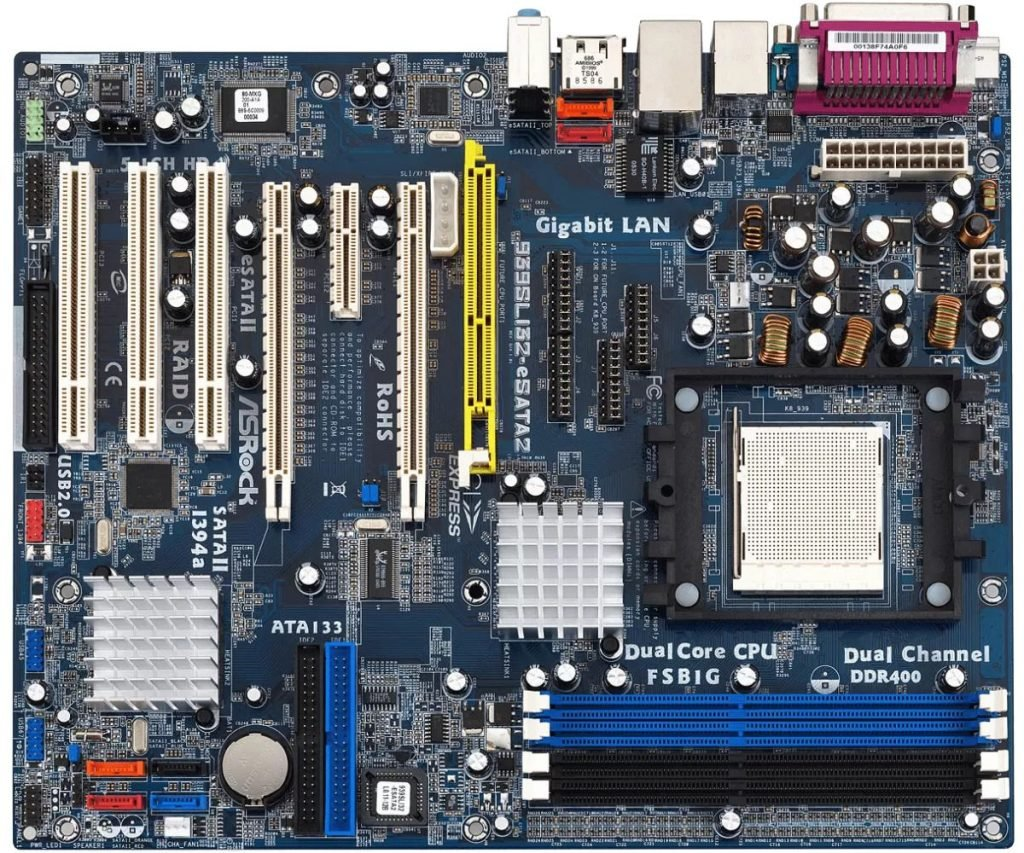
\includegraphics[width=0.65\linewidth]{Images/img8.jpg}
		\caption{Real NB and SB}
		\label{real NB and SB}
	\end{figure}
\end{frame}

%------------------------------------------------

\subsection{Chipsets}

\begin{frame}
	\frametitle{Chipsets}
	PCH chip in Z97 pro motherboard:
	\begin{figure}
		\centering
		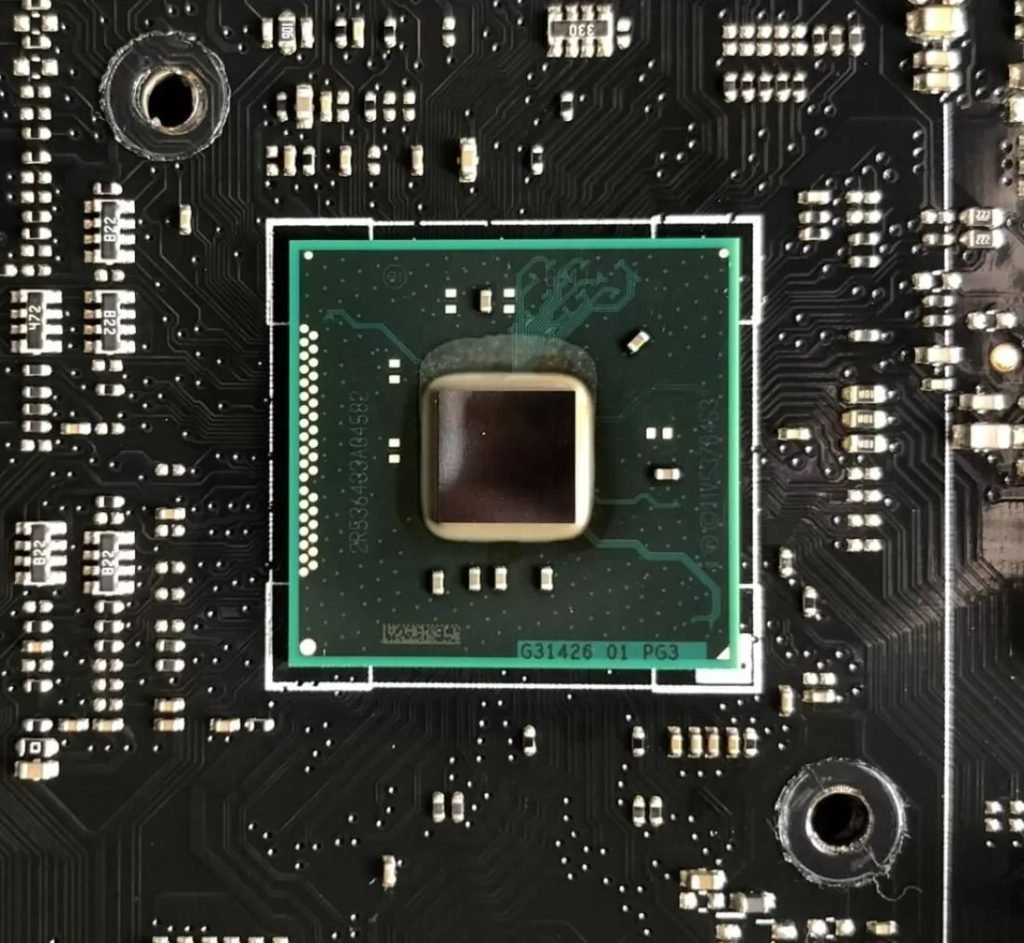
\includegraphics[width=0.5\linewidth]{Images/img9.jpg}
		\caption{PCH chip of Z97 pro}
		\label{PCH chip of Z97 pro}
	\end{figure}
\end{frame}

%------------------------------------------------

\subsection{Power section}

\begin{frame}
	\frametitle{Power section}
	\textcolor{blue}{P}ower \textcolor{blue}{S}upply \textcolor{blue}{U}nit or PSU provides the voltage and current of the board using a 24-pin connector called \textcolor{blue}{ATX}.
	
	\begin{figure}
		\centering
		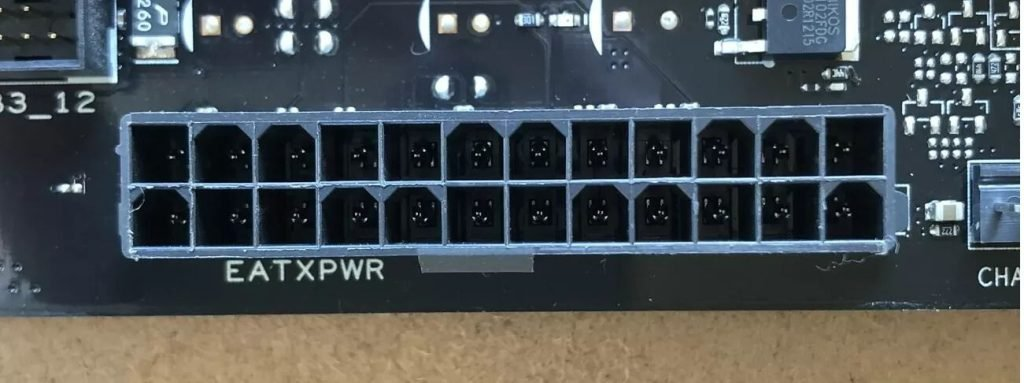
\includegraphics[width=0.8\linewidth]{Images/img10.jpg}
		\caption{ATX connector}
		\label{atx connector}
	\end{figure}
\end{frame}




\begin{frame}
	\frametitle{Power section}
	In today's motherboards, there is another 8-pin output in the power supply unit.
	
	\begin{figure}
		\centering
		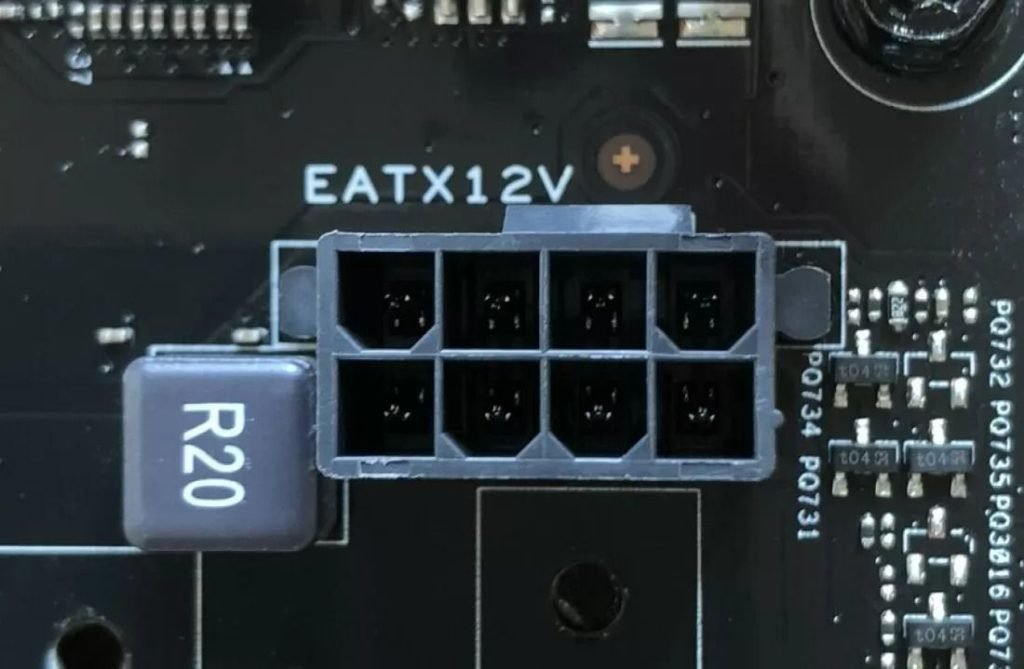
\includegraphics[width=0.7\linewidth]{Images/img11.jpg}
		\caption{ATX connector}
		\label{atx8 connector}
	\end{figure}
\end{frame}




\begin{frame}
	\frametitle{Power section}
	\framesubtitle{Figure}
	In this figure, you can see the output voltages of these two connectors:
	
	\begin{figure}
		\centering
		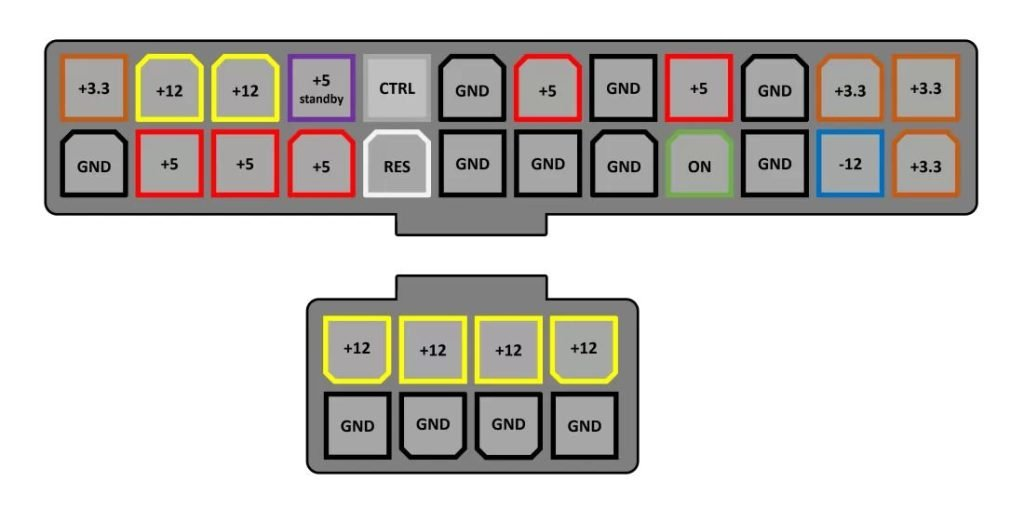
\includegraphics[width=0.8\linewidth]{Images/img12.jpg}
		\caption{ATX output schematic}
		\label{ATX output schematic}
	\end{figure}
\end{frame}





\begin{frame}
	\frametitle{Power section}
	\framesubtitle{Gray area!}
	\textbf{In what voltage range do today's CPUs work?}
	\begin{itemize}
		\item Today's CPUs doesn't work with constant voltage.
		\item less than 0.8 volts when in low power mode.
		\item 1.4 volts or more in full power mode.
	\end{itemize}
	
	\bigskip
	
	Therefore, there must be a unit in the motherboard that reduces the 12 V output voltage of the PSU to this range.
	
	\bigskip
	
	\alert{This unit is called \textcolor{blue}{V}oltage \textcolor{blue}{R}egulation \textcolor{blue}{M}odules or VRM}
	
\end{frame}



%------------------------------------------------

\section{Today's technology}

\subsection{Manufacturing companies}

\begin{frame}
	\frametitle{Manufacturing companies}
	Top motherboard manufacturers:
	\begin{enumerate}
		\item ASRock
		\item Asus
		\item Biostar
		\item EVGA Corporation
		\item Gigabyte Technology
		\item MSI (Micro-Star International)
		\item Intel
	\end{enumerate}
\end{frame}

%------------------------------------------------

\subsection{Types of motherboard}

\begin{frame}
	\frametitle{Types of motherboard}
	Here are some common types of motherboards:
	\begin{enumerate}
		\item ATX \textit{(Advanced Technology eXtended)	}
		\item Micro ATX
		\item Mini ITX
		\item Extended ATX
		\item ITX
		\item BTX
	\end{enumerate}
\end{frame}

%------------------------------------------------

\begin{frame} % Use [allowframebreaks] to allow automatic splitting across slides if the content is too long
	\frametitle{References}
	
	\begin{thebibliography}{99} % Beamer does not support BibTeX so references must be inserted manually as below, you may need to use multiple columns and/or reduce the font size further if you have many references
		\footnotesize % Reduce the font size in the bibliography
		
		\bibitem[Digiato]{p1}
			Digiato: \href{https://digiato.com/}{link}
			
		\bibitem[Wikipedia]{p2}
			Wikipedia: \href{https://www.wikipedia.org/}{link}
	\end{thebibliography}
\end{frame}

%----------------------------------------------------------------------------------------
%	CLOSING SLIDE
%----------------------------------------------------------------------------------------

\begin{frame}[plain] % The optional argument 'plain' hides the headline and footline
	\begin{center}
		{\Huge The End}
		
		\bigskip\bigskip % Vertical whitespace
		
		{\LARGE Questions? Comments?}
	\end{center}
\end{frame}

%----------------------------------------------------------------------------------------

\end{document} 